\chapter{Návrhové obrazovky}\label{appendix:navrhoveObrazovky}



\begin{figure}[ht!]
    \centering
    \includegraphics[width=0.9\textwidth,page=1]{media/04_navrh/navhoveObrazovky.pdf}
    \caption{Návrhová obrazovka přihlašovací stránky v záložce \enquote{E-mail a heslo}}
\end{figure}

\begin{figure}[ht!]
    \centering
    \includegraphics[width=0.95\textwidth,page=2]{media/04_navrh/navhoveObrazovky.pdf}
    \caption{Návrhová obrazovka přihlašovací stránky v záložce \enquote{E-mail s potvrzením}}
\end{figure}

\begin{figure}[ht!]
    \centering
    \includegraphics[width=0.95\textwidth,page=12]{media/04_navrh/navhoveObrazovky.pdf}
    \caption{Návrhová obrazovka přihlašovací stránky v záložce \enquote{E-mail s potvrzením} po odeslání žádosti}
\end{figure}



\begin{figure}[ht!]
    \centering
    \includegraphics[width=0.95\textwidth,page=3]{media/04_navrh/navhoveObrazovky.pdf}
    \caption{Návrhová obrazovka stránky s registračním formulářem}
\end{figure}

\begin{figure}[ht!]
    \centering
    \includegraphics[width=0.95\textwidth,page=4]{media/04_navrh/navhoveObrazovky.pdf}
    \caption{Návrhová obrazovka po úspěšném zaregistrování účtu}
\end{figure}

\begin{figure}[ht!]
    \centering
    \includegraphics[width=0.95\textwidth,page=5]{media/04_navrh/navhoveObrazovky.pdf}
    \caption{Návrhová obrazovka hlavního panelu s materiály uživatele}
\end{figure}

\begin{figure}[ht!]
    \centering
    \includegraphics[width=0.95\textwidth,page=13]{media/04_navrh/navhoveObrazovky.pdf}
    \caption{Návrhová obrazovka vyskakovacího okna s novým materiálem a importováním materiálu}
\end{figure}

\begin{figure}[ht!]
    \centering
    \includegraphics[width=0.95\textwidth,page=18]{media/04_navrh/navhoveObrazovky.pdf}
    \caption{Návrhová obrazovka vyskakovacího okna s importováním materiálu, výběrem souboru a chybou}
\end{figure}


\begin{figure}[ht!]
    \centering
    \includegraphics[width=0.95\textwidth,page=6]{media/04_navrh/navhoveObrazovky.pdf}
    \caption{Návrhová obrazovka s vytvořenými rozšířeními uživatele}
\end{figure}

\begin{figure}[ht!]
    \centering
    \includegraphics[width=0.95\textwidth,page=14]{media/04_navrh/navhoveObrazovky.pdf}
    \caption{Návrhová obrazovka vyskakovacího okna s přehledem verzí konkrétního rozšíření}
\end{figure}


\begin{figure}[ht!]
    \centering
    \includegraphics[width=0.95\textwidth,page=7]{media/04_navrh/navhoveObrazovky.pdf}
    \caption{Návrhová obrazovka s nastavením uživatele}
\end{figure}

\begin{figure}[ht!]
    \centering
    \includegraphics[width=0.95\textwidth,page=8]{media/04_navrh/navhoveObrazovky.pdf}
    \caption{Návrhová obrazovka editoru s blokem textu}
\end{figure}

\begin{figure}[ht!]
    \centering
    \includegraphics[width=0.95\textwidth,page=15]{media/04_navrh/navhoveObrazovky.pdf}
    \caption{Návrhová obrazovka editoru s otevřeným panelem snímků}
\end{figure}


\begin{figure}[ht!]
    \centering
    \includegraphics[width=0.95\textwidth,page=20]{media/04_navrh/navhoveObrazovky.pdf}
    \caption{Návrhová obrazovka editoru s otevřeným panelem k přidání bloku}
\end{figure}


\begin{figure}[ht!]
    \centering
    \includegraphics[width=0.95\textwidth,page=21]{media/04_navrh/navhoveObrazovky.pdf}
    \caption{Návrhová obrazovka editoru s otevřeným panelem k přidání vlastního multimédia}
\end{figure}


\begin{figure}[ht!]
    \centering
    \includegraphics[width=0.95\textwidth,page=9]{media/04_navrh/navhoveObrazovky.pdf}
    \caption{Návrhová obrazovka editoru s otevřeným panelem vlastností bloku}
\end{figure}


\begin{figure}[ht!]
    \centering
    \includegraphics[width=0.95\textwidth,page=10]{media/04_navrh/navhoveObrazovky.pdf}
    \caption{Návrhová obrazovka editoru s otevřeným vyskakovacím oknem nastavením preferencí}
\end{figure}

\begin{figure}[ht!]
    \centering
    \includegraphics[width=0.95\textwidth,page=16]{media/04_navrh/navhoveObrazovky.pdf}
    \caption{Návrhová obrazovka editoru s otevřeným vyskakovacím oknem nastavením sdílení}
\end{figure}

\begin{figure}[ht!]
    \centering
    \includegraphics[width=0.95\textwidth,page=21]{media/04_navrh/navhoveObrazovky.pdf}
    \caption{Návrhová obrazovka editoru s otevřeným vyskakovacím oknem s aktivními rozšířeními}
\end{figure}

\begin{figure}[ht!]
    \centering
    \includegraphics[width=0.95\textwidth,page=22]{media/04_navrh/navhoveObrazovky.pdf}
    \caption{Návrhová obrazovka editoru s otevřeným vyskakovacím oknem s přehledem možných rozšíření}
\end{figure}

\begin{figure}[ht!]
    \centering
    \includegraphics[width=0.95\textwidth,page=11]{media/04_navrh/navhoveObrazovky.pdf}
    \caption{Návrhová obrazovka přehrávače}
\end{figure}

\begin{figure}[ht!]
    \centering
    \includegraphics[width=0.95\textwidth,page=17]{media/04_navrh/navhoveObrazovky.pdf}
    \caption{Návrhová obrazovka přehrávače se zapnutým modem kreslení a kresbou}
\end{figure}




\chapter{Uživatelské rozhraní}\label{appendix:uzivatelskeRozhrani}


\begin{figure}[ht!]
    \centering
    \includegraphics[width=1\textwidth,page=9]{text/uzivatelskeProstredi.pdf}
    \caption{Uživatelské rozhraní hlavní stránky v tmavém režimu}
\end{figure}


\begin{figure}
\centering
\begin{minipage}{.4\textwidth}
  \centering
    \includegraphics[width=1\textwidth,page=10]{text/uzivatelskeProstredi.pdf}
    \captionof{figure}{Uživatelské rozhraní hlavní stránky na telefonním zařízení}
\end{minipage}%
\hspace{0.1\textwidth}
\begin{minipage}{.4\textwidth}
  \centering
    \includegraphics[width=1\textwidth,page=11]{text/uzivatelskeProstredi.pdf}
    \captionof{figure}[Uživatelské rozhraní hlavní stránky s otevřenou navigací]{Uživatelské rozhraní hlavní stránky na telefonním zařízení s otevřenou navigací}
\end{minipage}
\end{figure}

\chapter{Testovací scénáře}\label{appendix:testovaciScenare}

% TC-U: uživatel (user)
% TC-E: tvořitel v editoru
% TC-P: tvoritel v prehravaci
% TC-W: sledovatel (watcher) 

% TC-U-1 registrace
% TC-U-2 prihlaseni heslo
% TC-U-3 prihlaseni email
% TC-U-4 změna jazyka
% TC-U-5 změna nastaveni
% TC-U-6 export dat

% TC-E-1 vytvoreni prázdného materialu
% TC-E-2 manipulace s bloky + nastaveni vlastnosti
% TC-E-3 vlozeni vlastního obsahu
% TC-E-4 vlozeni obsahu z banky
% TC-E-5 práce se snímky

% TC-E-6 práce s editorem |||||| asi ne?

% TC-E-7 exportovani materialu JSON
% TC-E-8 exportovani materialu PDF
% TC-E-9 importovani materialu JSON
% TC-E-10 importovani materialu Markdown

% TC-E-11 nastaveni preferenci
% TC-E-12 nastaveni materialu

% TC-E-13 instalace a pouziti pluginu
% TC-E-14 odinstalovani pluginu

% TC-E-15 spusteni kolaborace, pouzivani
% TC-E-16 vytvoreni interaktivity 

% TC-E-17 oznaceni materilu jako vybraneho
% TC-E-18 oznaceni materialu jako nevybraneho

% TC-P-1 prochazeni materiálem
% TC-P-2 interakce s prvky
% TC-P-3 kresleni
% TC-P-4 sdileni
% TC-P-5 zapnuti sledovani

% TC-W-1 pripojeni se ke sledovani
% TC-W-2 interakce s interaktivními bloky

\vspace{1em}\noindent{\large\textbf{TC-U-1 -- Vytvoření uživatelského účtu}}

\textbf{Cíl}: Účelem je vytvoření uživatelského účtu uvnitř vytvořené aplikace.

\textbf{Časový limit}: do 5 minut

\textbf{Podmínky}: Aplikace je ve stavu, kdy uživatel není přihlášen a uživatel se nachází na hlavní stránce aplikace. Uživatel nemá zaregistrovaný žádný účet.

\textbf{Kroky}:

\begin{enumerate}[leftmargin=1.4cm]
    \item Účastník klikne na tlačítko \verb|Vytvořit si účet|.
    \item Účastník vyplní registrační formulář.
    \item Účastník formulář odešle kliknutím na tlačítko \verb|Registrovat se|.
    \item Účastník zkontroluje svoji e-mailovou schránku pro e-mail obsahující informace o aktivaci.
    \item Účastník si pomocí pokynů z e-mailu aktivuje účet.
\end{enumerate}

\textbf{Očekávané výsledky}:

\begin{enumerate}[leftmargin=1.4cm]
    \item Aplikace ho přesměruje automaticky na stránku s přihlášením.
    \item V aplikaci se vytvořil nový účet se zadanými údaji.
    \item Na zadaný e-mail aplikace odeslala e-mail se žádostí o potvrzení e-mailu a aktivaci účtu.
    \item Účet je aktivovaný a lze se do něj přihlásit.
\end{enumerate}


\vspace{1em}\noindent{\large\textbf{TC-U-2 -- Přihlášení se pomocí e-mailu a hesla}}

\textbf{Cíl}: Účelem je přihlásit se do již existujícího účtu v aplikaci pomocí e-mailu a hesla.

\textbf{Časový limit}: do 5 minut

\textbf{Podmínky}: Aplikace je ve stavu, kdy uživatel není přihlášen a uživatel se nachází na hlavní stránce. Účet již má účastník vytvořený a ví jeho přihlašovací údaje, například dle TC-U-1.

\textbf{Kroky}:

\begin{enumerate}[leftmargin=1.4cm]
    \item Účastník klikne na tlačítko \verb|E-mail a heslo|.
    \item Účastník vyplní svůj e-mail a heslo.
    \item Účastník formulář odešle kliknutím na tlačítko \verb|Přihlásit se|.
\end{enumerate}

\textbf{Očekávané výsledky}:

\begin{enumerate}[leftmargin=1.4cm]
    \item Aplikace ho přesměruje automaticky na stránku s přihlášením.
    \item Uživatel je přihlášen.
    \item Je zobrazena hlavní stránka s informacemi o přihlášeném uživateli.
\end{enumerate}


\vspace{1em}\noindent{\large\textbf{TC-U-3 -- Přihlášení se pomocí e-mail s potvrzením}}

\textbf{Cíl}: Účelem je přihlásit se do již existujícího účtu v aplikaci pomocí e-mailu s potvrzením.

\textbf{Časový limit}: do 5 minut

\textbf{Podmínky}: Aplikace je ve stavu, kdy uživatel není přihlášen a uživatel se nachází na hlavní stránce. Účet již má účastník vytvořený a ví jeho přihlašovací údaje, například dle TC-U-1.

\textbf{Kroky}:

\begin{enumerate}[leftmargin=1.4cm]
    \item Účastník zvolí možnost přihlášení pomocí e-mailu s potvrzením.
    \item Účastník vyplní formulář s e-mailem.
    \item Účastník formulář odešle pomocí kliknutí na tlačítko \verb|Přihlásit se|.
    \item Účastník si své své e-mailovou schránce vyzvedne informace o přihlášení.
    \item Účastník do formuláře (či na nové stránce) vyplní kód, který mu přišel e-mailem.
    \item Účastník formulář odešle pomocí kliknutí na tlačítko \verb|Přihlásit se|.
\end{enumerate}

\textbf{Očekávané výsledky}:

\begin{enumerate}[leftmargin=1.4cm]
    \item Aplikace ho přesměruje automaticky na stránku s přihlášením.
    \item Uživatel je přihlášen.
    \item Je zobrazena hlavní stránka s informacemi o přihlášeném uživateli.
\end{enumerate}


\vspace{1em}\noindent{\large\textbf{TC-U-4 -- Změna jazyka}}

\textbf{Cíl}: Účelem je, aby si uživatel v aplikaci změnil jazyk na jiný.

\textbf{Časový limit}: do 2 minut

\textbf{Podmínky}: Aplikace je na nějaké stránce z množiny: hlavní stránka, editor, přehrávač, přihlášení.

\textbf{Kroky}:

\begin{enumerate}[leftmargin=1.4cm]
    \item Účastník v aplikaci nalezne tlačítko v horní navigaci s ikonou překladů.
    \item Účastník na tlačítko klikne a poté z vyskakovacího menu vybere jiný jazyk, než je aktuálně nastaven.
\end{enumerate}

\textbf{Očekávané výsledky}:

\begin{enumerate}[leftmargin=1.4cm]
    \item V aplikaci se změní jazyk na nově vybraný a všechny texty budou přeloženy v daném jazyce.
\end{enumerate}






\vspace{1em}\noindent{\large\textbf{TC-U-5 -- Změna údajů účtu}}

\textbf{Cíl}: Uživatel si změn své jméno a heslo v aplikaci.

\textbf{Časový limit}: do 5 minut

\textbf{Podmínky}: Uživatel je v aplikaci přihlášen a zná svoje přihlašovací údaje. Uživatel je na panelu materiálů.

\textbf{Kroky}:

\begin{enumerate}[leftmargin=1.4cm]
    \item Uživatel nalezne tlačítko \verb|Nastavení| v horní navigaci.
    \item Uživatel tlačítko zmáčkne a do formuláře zadá dle svého uvážení nové jméno a nové heslo v aplikaci.
    \item Uživatel zadá své aktuálního heslo.
    \item Uživatel klikne na tlačítko \verb|Změnit údaje|.
    \item Poté uživatel přistoupí na hlavní stránku, kde nové údaje ověří.
\end{enumerate}

\textbf{Očekávané výsledky}:

\begin{enumerate}[leftmargin=1.4cm]
    \item Ve formuláři bylo automaticky vyplněno aktuální jméno v aplikaci.
    \item Při správně zadaném aktuálním heslu se údaje změnily a jsou ihned vidět na hlavní stránce.
\end{enumerate}





\vspace{1em}\noindent{\large\textbf{TC-U-6 -- Exportování dat}}

\textbf{Cíl}: Uživatel si požádá o exportování osobních údajů a dat z aplikace a ty obdrží na e-mail.

\textbf{Časový limit}: do 5 minut

\textbf{Podmínky}: Uživatel je v aplikaci přihlášen a nachází se na hlavní stránce. Uživatel v nedávné době o export osobních údajů nežádal.

\textbf{Kroky}:

\begin{enumerate}[leftmargin=1.4cm]
    \item Uživatel nalezne tlačítko \verb|Nastavení| v horní navigaci.
    \item Uživatel tlačítko zmáčkne a ve formuláři pro export si přečte informace.
    \item Potom požádá o export osobních údajů a dat stiskem na tlačítko \verb|Zažádat o export|.
    \item Uživatel počká na zpracování a čeká ve své e-mailové schránce.
    \item Uživatel přistoupí na stejnou stránku a pomocí tlačítka \verb|Stáhnout| obdrží archív s osobními údaji.
    \item Uživatel si na počítači archív otevře a prozkoumá jejich obsah.
\end{enumerate}

\textbf{Očekávané výsledky}:

\begin{enumerate}[leftmargin=1.4cm]
    \item Aplikace požadavek zpracuje a odešle e-mail.
    \item Stáhnutý archív bude obsahovat minimálně dva soubory  \verb|user.json| a \verb|preferences.json| s údaji uživatele z aplikace.
\end{enumerate}

\textbf{Poznámky}:

\begin{itemize}[leftmargin=1.4cm]
    \item Aplikace nemusí stihnout v reálném čase požadavek zpracovat, testovací verze aplikace musí mít vypnutý zpomalovač požadavků a případně tomuto exportu dát větší prioritu.
\end{itemize}






\vspace{1em}\noindent{\large\textbf{TC-E-1 -- Vytvoření prázdného materiálu}}

\textbf{Cíl}: Uživatel v aplikaci vytvoří nový materiál bez obsahu.

\textbf{Časový limit}: do 2 minut

\textbf{Podmínky}: Uživatel je v aplikaci přihlášen a nachází se na hlavní stránce.

\textbf{Kroky}:

\begin{enumerate}[leftmargin=1.4cm]
    \item Uživatel naleznete tlačítko přidání materiálu pod ikonou znaku plus.
    \item Uživatel na tlačítko klikne a uvnitř vyskakovacího okna vybere možnost nového materiálu.
    \item Uživatel v editoru klikne na tlačítko panelu a na hlavní stránce znovu otevře stejný materiál.
\end{enumerate}

\textbf{Očekávané výsledky}:

\begin{enumerate}[leftmargin=1.4cm]
    \item Aplikace vytvoří prázdný materiál a uživatele na něj přesměruje.
    \item Materiál bude k dispozici na hlavní stránce.
\end{enumerate}






\vspace{1em}\noindent{\large\textbf{TC-E-2 -- Tvorba bloků a jejich manipulace}}

\textbf{Cíl}: Uživatel v materiálu přidá základní bloky -- text a tvar. Bloky umístí do editoru. Textu změní obsah, barvu a podtržení. Bloku tvaru změní tvar a barvu. Tvar otočí o 90 stupňů a zvětší ho. 

\textbf{Časový limit}: do 10 minut

\textbf{Podmínky}:  Uživatel je v aplikaci přihlášen a nachází se na hlavní stránce. Uživatel má vytvořený prázdný materiál, jako například v TC-E-1.

\textbf{Kroky}:

\begin{enumerate}[leftmargin=1.4cm]
    \item Účastník na hlavní stránce otevře materiál klikem na jeho kartičku.
    \item Účastník v editoru nalezne panel pro přidávání bloků s ikonou plus ve čtverci.
    \item Účastník do editoru přidá blok tvaru a textu.
    \item Účastník upraví text dvojklikem na něm.
    \item Účastník označí v textu slova a jim změní pomocí postranního panelu s vlastnostmi barvu a podtržení.
    \item Účastník označí blok, v panelu vlastností změní tvar a barvu.
    \item Účastník pomocí panelu vlastností či pomocí nástrojů uvnitř editoru změní rotaci a velikost.
\end{enumerate}

\textbf{Očekávané výsledky}:

\begin{enumerate}[leftmargin=1.4cm]
    \item Na prvním snímku v materiálu je blok textu a tvaru.
    \item Text má vlastní obsah, který je obarven a podtržen.
    \item Tvar je pootočen, zvětšen, je obarven a má nastaven nějaký tvar. 
\end{enumerate}






\vspace{1em}\noindent{\large\textbf{TC-E-3 -- Přidání vlastního obsahu}}

\textbf{Cíl}: Uživatel v materiálu nahraje vlastní obrázek a ten vloží do materiálu.

\textbf{Časový limit}: do 5 minut

\textbf{Podmínky}:  Uživatel je v aplikaci přihlášen a nachází se na hlavní stránce. Uživatel má vytvořený prázdný materiál, jako například v TC-E-1. Uživatel má na počítači obrázek, který nahraje do aplikace.

\textbf{Kroky}:

\begin{enumerate}[leftmargin=1.4cm]
    \item Účastník na hlavní stránce otevře materiál klikem na jeho kartičku.
    \item Účastník v editoru nalezne panel pro přidávání obsahu s ikonou multimédií.
    \item V postranním panelu uživatel klikne na tlačítko \verb|Nahrát obsah|.
    \item Účastník v počítači vybere soubor a nahraje ho.
    \item Účastník v postranním menu obrázek vybere a přidá ho do materiálu.
\end{enumerate}

\textbf{Očekávané výsledky}:

\begin{enumerate}[leftmargin=1.4cm]
    \item Na prvním snímku v materiálu je nový blok s obrázkem od uživatele.
    \item Obrázek se nahrál do aplikace.
\end{enumerate}






\vspace{1em}\noindent{\large\textbf{TC-E-4 -- Přidání obsahu z banky}}

\textbf{Cíl}: Uživatel v materiálu nahraje obrázek z banky obsahu.

\textbf{Časový limit}: do 5 minut

\textbf{Podmínky}:  Uživatel je v aplikaci přihlášen a nachází se na hlavní stránce. Uživatel má vytvořený prázdný materiál, jako například v TC-E-1.

\textbf{Kroky}:

\begin{enumerate}[leftmargin=1.4cm]
    \item Účastník na hlavní stránce otevře materiál klikem na jeho kartičku.
    \item Účastník v editoru nalezne panel pro přidávání obsahu s ikonou glóbusu.
    \item V postranním panelu uživatel vybere, zda chce nahrávat obrázek či animovaný GIF.
    \item Účastník v postranním panelu vybere obrázek či animovaný GIF a přidá ho do materiálu.
\end{enumerate}

\textbf{Očekávané výsledky}:

\begin{enumerate}[leftmargin=1.4cm]
    \item Na prvním snímku v materiálu je nový blok s vybraným obrázkem od uživatele z banky animovaných GIF či obrázků.
\end{enumerate}






\vspace{1em}\noindent{\large\textbf{TC-E-5 -- Práce se snímky}}

\textbf{Cíl}: Uživatel v materiálu přidá dva další snímky, změní jim pozadí a velikost, a do každého snímku vloží nějaký obsah.

\textbf{Časový limit}: do 5 minut

\textbf{Podmínky}:  Uživatel je v aplikaci přihlášen a nachází se na hlavní stránce. Uživatel má vytvořený prázdný materiál, jako například v TC-E-1.

\textbf{Kroky}:

\begin{enumerate}[leftmargin=1.4cm]
    \item Účastník na hlavní stránce otevře materiál klikem na jeho kartičku.
    \item Účastník v editoru nalezne panel snímků s ikonou kartiček.
    \item V postranním panelu účastník klikne na tlačítko \verb|Přidat snímek| dvakrát.
    \item V postranním panelu účastník otevře nastavení snímku a změní jim barvu pozadí a jejich velikost.
    \item Účastník prochází mezi snímky a do každého z nich vloží obsah.
\end{enumerate}

\textbf{Očekávané výsledky}:

\begin{enumerate}[leftmargin=1.4cm]
    \item Materiál má vytvořené tři snímky, kde v každém z nich je jiný obsah, mají jiné pozadí a jinou velikost.
\end{enumerate}






\vspace{1em}\noindent{\large\textbf{TC-E-6 -- Exportování materiálu do JSON}}

\textbf{Cíl}: Uživatel exportuje materiál do formátu JSON pomocí aplikace.

\textbf{Časový limit}: do 2 minut

\textbf{Podmínky}:  Uživatel je v aplikaci přihlášen a nachází se na hlavní stránce. Uživatel má vytvořený materiál s nějakým obsahem, stejně jako například po TC-E-5.

\textbf{Kroky}:

\begin{enumerate}[leftmargin=1.4cm]
    \item Účastník na hlavní stránce otevře materiál klikem na jeho kartičku.
    \item Účastník v horním navigaci najde tlačítko \verb|Sdílení| a klikne na něj.
    \item Účastník vybere možnost \verb|Export materiálu| a poté vybere možnost \verb|JSON|.
    \item Účastník ověří, že soubor není prázdný tím, že ho otevře.
\end{enumerate}

\textbf{Očekávané výsledky}:

\begin{enumerate}[leftmargin=1.4cm]
    \item Materiál se automaticky stáhne pod názvem materiálu s příponou \verb|.json|.
\end{enumerate}




\vspace{1em}\noindent{\large\textbf{TC-E-7 -- Exportování materiálu do PDF}}

\textbf{Cíl}: Uživatel exportuje materiál do formátu PDF pomocí aplikace.

\textbf{Časový limit}: do 10 minut

\textbf{Podmínky}:  Uživatel je v aplikaci přihlášen a nachází se na hlavní stránce. Uživatel má vytvořený materiál s nějakým obsahem, stejně jako například po TC-E-5.

\textbf{Kroky}:

\begin{enumerate}[leftmargin=1.4cm]
    \item Účastník na hlavní stránce otevře materiál klikem na jeho kartičku.
    \item Účastník v horním navigaci najde tlačítko \verb|Sdílení| a klikne na něj.
    \item Účastník vybere možnost \verb|Export materiálu| a poté vybere možnost \verb|PDF|.
    \item Účastník ověří, že soubor není prázdný tím, že ho otevře.
\end{enumerate}

\textbf{Očekávané výsledky}:

\begin{enumerate}[leftmargin=1.4cm]
    \item Materiál se automaticky stáhne pod názvem materiálu s příponou \verb|.pdf|.
    \item Vytvořený soubor obsahuje přesnou kopii vytvořených prvků s danou vizualizací a velikostmi.
\end{enumerate}

\textbf{Poznámky}:

\begin{itemize}[leftmargin=1.4cm]
    \item Aplikace nemusí stihnout v reálném čase požadavek zpracovat, protože exportování závisí na využití vykreslovače na serveru.
\end{itemize}





\vspace{1em}\noindent{\large\textbf{TC-E-8 -- Importování materiálu z JSON}}

\textbf{Cíl}: Uživatel do aplikace importuje materiál z formátu JSON.

\textbf{Časový limit}: do 5 minut

\textbf{Podmínky}:  Uživatel je v aplikaci přihlášen a nachází se na hlavní stránce. Uživatel má stáhnutou zálohu jiného materiálu, například dle scénáře TC-E-6.

\textbf{Kroky}:

\begin{enumerate}[leftmargin=1.4cm]
    \item Uživatel naleznete tlačítko přidání materiálu pod ikonou znaku plus.
    \item Uživatel na tlačítko klikne a uvnitř vyskakovacího okna vybere možnost importu materiálu.
    \item Účastník v počítači vybere soubor a nahraje ho.
    \item Účastník projde vytvořený materiál zda souhlasí s exportovanou verzí.
\end{enumerate}\todo{vsude opravit účastník/uživatel}

\textbf{Očekávané výsledky}:

\begin{enumerate}[leftmargin=1.4cm]
    \item Materiál se vytvořil dle přiloženého souboru typu JSON.
\end{enumerate}






\vspace{1em}\noindent{\large\textbf{TC-E-9 -- Importování materiálu z Markdown}}

\textbf{Cíl}: Uživatel do aplikace importuje materiál z formátu Markdown.

\textbf{Časový limit}: do 10 minut

\textbf{Podmínky}:  Uživatel je v aplikaci přihlášen a nachází se na hlavní stránce. Uživatel ví, jak vypadá formát JSON a je schopný ho samostatně napsat.

\textbf{Kroky}:

\begin{enumerate}[leftmargin=1.4cm]
    \item Uživatel naleznete tlačítko přidání materiálu pod ikonou znaku plus.
    \item Uživatel na tlačítko klikne a uvnitř vyskakovacího okna vybere možnost importu materiálu.
    \item Uživatel si na počítači založí soubor s příponou \verb|md|.
    \item Uživatel dle pokynů vytvoří nějakou strukturu prezentace za pomocí nadpisu H1, H2 a textových tagů jak je list, tučné písmo, podtržení a další.
    \item Účastník v počítači vybere soubor a nahraje ho.
    \item Účastník projde vytvořený materiál zda souhlasí s tím, co uvedl v souboru.
\end{enumerate}

\textbf{Očekávané výsledky}:

\begin{enumerate}[leftmargin=1.4cm]
    \item Materiál se vytvořil dle přiloženého souboru typu Markdown a obsahuje vše, co uživatel zadal.
\end{enumerate}





\vspace{1em}\noindent{\large\textbf{TC-E-10 -- Nastavení preferencí}}

\textbf{Cíl}: Uživatel si změní preference v editoru a vyzkouší změněné možnosti.

\textbf{Časový limit}: do 5 minut

\textbf{Podmínky}:  Uživatel je v aplikaci přihlášen a nachází se na hlavní stránce.  Uživatel má vytvořený materiál s nějakým obsahem, stejně jako například po TC-E-5.

\textbf{Kroky}:

\begin{enumerate}[leftmargin=1.4cm]
    \item Účastník na hlavní stránce otevře materiál klikem na jeho kartičku.
    \item Účastník v horním navigaci najde tlačítko \verb|Předvolby| a klikne na něj.
    \item Účastník si přečte možnosti nastavení a dle svého uvážení ho upraví. 
    \item Účastník klikem na tlačítko \verb|Uložit| uloží své nastavení.
    \item Změněné nastavení účastník vyzkouší přímo v editoru.
\end{enumerate}

\textbf{Očekávané výsledky}:

\begin{enumerate}[leftmargin=1.4cm]
    \item Uživatelské předvolby a preference editoru se změnily a propsali se do aktuálně otevřeného editoru. 
\end{enumerate}




\vspace{1em}\noindent{\large\textbf{TC-E-11 -- Nastavení materiálu}}

\textbf{Cíl}: Uživatel si pro materiál změní nastavení. Změní jméno, viditelnost, průchod a zobrazení materiálu.

\textbf{Časový limit}: do 5 minut

\textbf{Podmínky}:  Uživatel je v aplikaci přihlášen a nachází se na hlavní stránce.  Uživatel má vytvořený materiál s nějakým obsahem, stejně jako například po TC-E-5.

\textbf{Kroky}:

\begin{enumerate}[leftmargin=1.4cm]
    \item Účastník na hlavní stránce otevře materiál klikem na jeho kartičku.
    \item Účastník v horním navigaci najde tlačítko \verb|Sdílení| a klikne na něj.
    \item Poté zvolí možnost \verb|Nastavení materiálu|.
    \item Účastník si přečte možnosti nastavení a dle svého uvážení je upraví. 
    \item Účastník klikem na tlačítko \verb|Uložit| uloží své nastavení.
    \item Změněné nastavení účastník vyzkouší přímo v přehrávači.
\end{enumerate}

\textbf{Očekávané výsledky}:

\begin{enumerate}[leftmargin=1.4cm]
    \item Nastavení materiálu se změnilo na vyplněné hodnoty.
    \item Pokud uživatel nastavil materiál jako veřejný, je možné ho navštívit se odkazem pro sdílení.
\end{enumerate}




\vspace{1em}\noindent{\large\textbf{TC-E-12 -- Instalace a použití rozšíření}}

\textbf{Cíl}: Uživatel si v materiálu nainstaluje rozšíření \verb|Word wall| a použije ho. Tedy přidá blok do materiálu.

\textbf{Časový limit}: do 5 minut

\textbf{Podmínky}:  Uživatel je v aplikaci přihlášen a nachází se na hlavní stránce.  Uživatel má vytvořený prázdný materiál. V aplikaci se nachází ukázkové rozšíření \verb|Word wall|.

\textbf{Kroky}:

\begin{enumerate}[leftmargin=1.4cm]
    \item Účastník na hlavní stránce otevře materiál klikem na jeho kartičku.
    \item Účastník v boční navigaci najde tlačítko \verb|Spravovat pluginy| a klikne na něj.
    \item Poté zvolí možnost \verb|Procházet pluginy|.
    \item Účastník vybere a nainstaluje rozšíření \verb|Word wall|.
    \item Účastník v navigaci pod rozšířením otevře panel rozšíření a zvolí možnost přidání bloku do materiálu.
    \item Účastník vyzkouší rozšíření přímo v přehrávači.
\end{enumerate}

\textbf{Očekávané výsledky}:

\begin{enumerate}[leftmargin=1.4cm]
    \item Materiál nyní obsahuje nainstalované rozšíření nejnovější možné verze.
    \item Materiál obsahuje vlastní blok pluginu a rozšíření s blokem funguje.
\end{enumerate}



\vspace{1em}\noindent{\large\textbf{TC-E-13 -- Odinstalování rozšíření}}

\textbf{Cíl}: Uživatel si v materiálu odinstaluje rozšíření \verb|Word wall|.

\textbf{Časový limit}: do 5 minut

\textbf{Podmínky}:  Aplikace je v stavu po provedení scénáře TC-E-13. Uživatel se nachází na stránce materiálu.

\textbf{Kroky}:

\begin{enumerate}[leftmargin=1.4cm]
    \item Účastník v boční navigaci najde tlačítko \verb|Spravovat pluginy| a klikne na něj.
    \item Účastník odinstaluje rozšíření \verb|Word wall|.
    \item Účastník odebere blok rozšíření z materiálu.
\end{enumerate}

\textbf{Očekávané výsledky}:

\begin{enumerate}[leftmargin=1.4cm]
    \item Materiál neobsahuje žádné nainstalované rozšíření.
\end{enumerate}




\vspace{1em}\noindent{\large\textbf{TC-E-14 -- Kolaborace}}

\textbf{Cíl}: Uživatel si v materiálu zapne kolaboraci a zkusí editovat materiál z dvou různých oken prohlížeče. 

\textbf{Časový limit}: do 5 minut

\textbf{Podmínky}:  Uživatel je v aplikaci přihlášen a nachází se na hlavní stránce.  Uživatel má vytvořený materiál s nějakým obsahem, stejně jako například po TC-E-5.

\textbf{Kroky}:

\begin{enumerate}[leftmargin=1.4cm]
    \item Účastník na hlavní stránce otevře materiál klikem na jeho kartičku.
    \item Účastník otevře stejnou stránku v jiném okně prohlížeče.
    \item Účastník provede změny na nějakém snímku v různých instancích aplikace.
    \item Účastník může zkontrolovat připojené uživatele pomocí tlačítka uživatelů v horní části navigace.
\end{enumerate}

\textbf{Očekávané výsledky}:

\begin{enumerate}[leftmargin=1.4cm]
    \item Materiál se otevře v obou oknech prohlížeče.
    \item Materiál lze upravovat z obou instancí a změny se v reálném čase propisují do druhého okna.
    \item Blok v snímku nejde upravovat oběma instancemi najednou.
\end{enumerate}





\vspace{1em}\noindent{\large\textbf{TC-E-15 -- Vytvoření interaktivity}}

\textbf{Cíl}: Uživatel si ve snímku v materiálu vytvoři na bloku tvaru interaktivitu: při kliku na daný tvar se otevře stránka materalist.com v novém okně.

\textbf{Časový limit}: do 5 minut

\textbf{Podmínky}:  Uživatel je v aplikaci přihlášen a nachází se na hlavní stránce.  Uživatel má vytvořený materiál s nějakým obsahem, stejně jako například po TC-E-5.

\textbf{Kroky}:

\begin{enumerate}[leftmargin=1.4cm]
    \item Účastník na hlavní stránce otevře materiál klikem na jeho kartičku.
    \item Účastník přidá blok tvaru.
    \item Účastník v panelu vlastností přidá interaktivitu a nastaví hodnoty:
    \begin{itemize}
        \item \textbf{Událost}: Kliknuto.
        \item \textbf{Akce}: Otevřít odkaz.
        \item \textbf{Odkaz}: https://materalist.com
        \item \textbf{Pouze}: Vždy.
    \end{itemize}
    \item Účastník vyzkouší interaktivitu v přehrávači.
\end{enumerate}

\textbf{Očekávané výsledky}:

\begin{enumerate}[leftmargin=1.4cm]
    \item Materiál obsahuje blok s danou interaktivitou.
    \item Po kliku na blok v přehrávači se otevře nová stránka s adresou materalit.com.
\end{enumerate}




\vspace{1em}\noindent{\large\textbf{TC-E-16 -- Označení materiálu jako ukázkového}}

\textbf{Cíl}: Uživatel si v aplikaci označí nějaký svůj materiál jako ukázkový, aby se zobrazil na ukázkových materiálů.

\textbf{Časový limit}: do 5 minut

\textbf{Podmínky}:  Uživatel je v aplikaci přihlášen a nachází se na hlavní stránce.  Uživatel má vytvořený materiál s nějakým obsahem, stejně jako například po TC-E-5.

\textbf{Kroky}:

\begin{enumerate}[leftmargin=1.4cm]
    \item Účastník na hlavní stránce otevře ukázkové materiály.
    \item Účastník najde tlačítko pro přidání, označeno ikonou tvaru plus.
    \item Účastník vybere materiál, který chce označit jako ukázkový a odešle formulář tlačítkem \verb|Přidat|.
    \item Účastník uvidí vybraný materiál v seznamu.
\end{enumerate}

\textbf{Očekávané výsledky}:

\begin{enumerate}[leftmargin=1.4cm]
    \item Materiál obsahuje blok s danou interaktivitou.
    \item Po kliku na blok v přehrávači se otevře nová stránka s adresou materalit.com.
\end{enumerate}

\textbf{Poznámky}:

\begin{itemize}[leftmargin=1.4cm]
    \item Aplikace v daný moment může nezpracovat žádost o umístění do ukázkových materiálů. Pro testování je vhodné vypnout prodlevu k umístění.
\end{itemize}





\vspace{1em}\noindent{\large\textbf{TC-E-17 -- Přidání spoluúčastníka editace}}

\textbf{Cíl}: Uživatel si v aplikaci přidá do svého materiálu spoluúčastníka editace.

\textbf{Časový limit}: do 5 minut

\textbf{Podmínky}:  Uživatel je v aplikaci přihlášen a nachází se na hlavní stránce.  Uživatel má vytvořený materiál s nějakým obsahem, stejně jako například po TC-E-5. V aplikaci existuje další účet, který lze do materiálu přidat (a ten pozorovatel testování předloží účastníkovi).

\textbf{Kroky}:

\begin{enumerate}[leftmargin=1.4cm]
    \item Účastník na hlavní stránce otevře materiál klikem na jeho kartičku.
    \item Účastník v horní navigaci vybere možnosti nastavení.
    \item Ve vyskakovacím okně vybere možnost editace spolu účastníku editace.
    \item Účastník zadá e-mail, který mu poskytne pozorovatel testování.
    \item Pozorovatel se připojí a zkusí práci s editorem.
\end{enumerate}

\textbf{Očekávané výsledky}:

\begin{enumerate}[leftmargin=1.4cm]
    \item Do materiálu se dostane testovací účet a může editovat jednotlivé snímky.
\end{enumerate}






\vspace{1em}\noindent{\large\textbf{TC-P-1 -- Procházení materiálu}}

\textbf{Cíl}: Uživatel si v aplikaci otevře materiál a bude ho procházet.

\textbf{Časový limit}: do 5 minut

\textbf{Podmínky}:  Uživatel je v aplikaci přihlášen a nachází se na hlavní stránce.  Uživatel má vytvořený materiál s nějakým obsahem, stejně jako například po TC-E-5.

\textbf{Kroky}:

\begin{enumerate}[leftmargin=1.4cm]
    \item Účastník na hlavní stránce otevře materiál klikem na jeho kartičku.
    \item V horní navigaci účastník najde tlačítko \verb|Náhled| a klikem na něj.
    \item Na stránce v přehrávači uživatel prochází materiálem tlačítky v navigaci, pomocí šipek na klávesnici nebo kliky na snímek.
\end{enumerate}

\textbf{Očekávané výsledky}:

\begin{enumerate}[leftmargin=1.4cm]
    \item Materiál se otevřel v přehrávači a lze ním procházet.
\end{enumerate}



\vspace{1em}\noindent{\large\textbf{TC-P-2 -- Interakce s prvky}}

\textbf{Cíl}: Uživatel si v aplikaci otevře materiál a bude manipulovat s prvkem s interaktivitou.

\textbf{Časový limit}: do 5 minut

\textbf{Podmínky}:  Uživatel je v aplikaci přihlášen a nachází se na hlavní stránce.  Uživatel má vytvořený materiál s nějakým obsahem a blokem s interaktivitou, stejně jako například po scénáři TC-E-15.

\textbf{Kroky}:

\begin{enumerate}[leftmargin=1.4cm]
    \item Účastník na hlavní stránce otevře materiál klikem na jeho kartičku.
    \item V horní navigaci účastník najde tlačítko \verb|Náhled| a klikem na něj.
    \item Na stránce v přehrávači uživatel prochází materiálem tlačítky v navigaci, pomocí šipek na klávesnici nebo kliky na snímek.
    \item Účastník najde blok s tvarem a interaktivitou a klikne na něj.
\end{enumerate}

\textbf{Očekávané výsledky}:

\begin{enumerate}[leftmargin=1.4cm]
    \item Materiál lze procházet a s blokem lze interagovat.
    \item Po kliknutí na materiál se otevře nová stránka materalist.com.
\end{enumerate}






\vspace{1em}\noindent{\large\textbf{TC-P-3 -- Kreslení}}

\textbf{Cíl}: Uživatel si v aplikaci otevře materiál a v přehrávači bude kreslit na snímek pomocí různých barev a velikostí.

\textbf{Časový limit}: do 5 minut

\textbf{Podmínky}:  Uživatel je v aplikaci přihlášen a nachází se na hlavní stránce.  Uživatel má vytvořený materiál s nějakým obsahem, stejně jako například po TC-E-5.

\textbf{Kroky}:

\begin{enumerate}[leftmargin=1.4cm]
    \item Účastník na hlavní stránce otevře materiál klikem na jeho kartičku.
    \item V horní navigaci účastník najde tlačítko \verb|Náhled| a klikem na něj.
    \item Na stránce v přehrávači uživatel nalezne tlačítko \verb|Kreslení| a klikne na něj.
    \item Pomocí možností v dolní navigaci na snímku uživatel mění velikost, barvy, stabilizaci a další.
    \item Účastník na snímku něco nakreslí a označí.
\end{enumerate}

\textbf{Očekávané výsledky}:

\begin{enumerate}[leftmargin=1.4cm]
    \item Materiál lze procházet a na plátno lze kreslit.
    \item Možnosti kreslení (barva, velikost, stabilizace, guma) fungují.
\end{enumerate}






\vspace{1em}\noindent{\large\textbf{TC-P-4 -- Sdílení materiálu}}

\textbf{Cíl}: Uživatel si v aplikaci otevře materiál a v přehrávači zkopíruje odkaz pro sdílení. Odkaz účastník vyzkouší v anonymním okně.

\textbf{Časový limit}: do 5 minut

\textbf{Podmínky}:  Uživatel je v aplikaci přihlášen a nachází se na hlavní stránce.  Uživatel má vytvořený materiál s nějakým obsahem, stejně jako například po TC-E-5. Materiál musí být nastaven jako veřejný.

\textbf{Kroky}:

\begin{enumerate}[leftmargin=1.4cm]
    \item Účastník na hlavní stránce otevře materiál klikem na jeho kartičku.
    \item V horní navigaci účastník najde tlačítko \verb|Náhled| a klikem na něj.
    \item Na stránce v přehrávači uživatel nalezne tlačítko \verb|Sdílení| a klikne na něj.
    \item Účastník zkopíruje odkaz.
    \item Účastník otevře anonymní okno a otevře v něm materiál z odkazu.
\end{enumerate}

\textbf{Očekávané výsledky}:

\begin{enumerate}[leftmargin=1.4cm]
    \item Materiál lze procházet.
    \item Účastníkovi se zkopíroval odkaz pro sdílení.
    \item Účastník v anonymním režimu v prohlížeči funguje zobrazení materiálu.
\end{enumerate}





\vspace{1em}\noindent{\large\textbf{TC-P-5 -- Zapnutí sledování}}

\textbf{Cíl}: Uživatel si v aplikaci otevře materiál a v přehrávači zkopíruje odkaz pro sdílení se sledováním. Odkaz účastník vyzkouší v anonymním okně.

\textbf{Časový limit}: do 5 minut

\textbf{Podmínky}:  Uživatel je v aplikaci přihlášen a nachází se na hlavní stránce.  Uživatel má vytvořený materiál s nějakým obsahem, stejně jako například po TC-E-5. Materiál musí být nastaven jako veřejný.

\textbf{Kroky}:

\begin{enumerate}[leftmargin=1.4cm]
    \item Účastník na hlavní stránce otevře materiál klikem na jeho kartičku.
    \item V horní navigaci účastník najde tlačítko \verb|Náhled| a klikem na něj.
    \item Na stránce v přehrávači uživatel nalezne tlačítko \verb|Sdílení| a klikne na něj.
    \item Účastník vybere možnost \verb|Sdílení odkazu pro sledování|.
    \item Účastník zkopíruje odkaz.
    \item Účastník otevře anonymní okno a otevře v něm materiál z odkazu.
    \item V původním okně se účastník zkusí pohybovat mezi snímky a zkusí něco nakreslit. 
\end{enumerate}

\textbf{Očekávané výsledky}:

\begin{enumerate}[leftmargin=1.4cm]
    \item Materiál lze procházet.
    \item Účastníkovi se zkopíroval odkaz pro sdílení se sledováním.
    \item Účastník v anonymním režimu v prohlížeči funguje zobrazení materiálu.
    \item Procházení snímku a kresba se synchronizuje od prezentujícího.
\end{enumerate}




\vspace{1em}\noindent{\large\textbf{TC-P-6 -- Připojení se k sledování}}

\textbf{Cíl}: Uživatel se pomocí odkazu od pozorovatele testování připojí ke sledování a zkouší funkcionality módu sledujícího.

\textbf{Časový limit}: do 5 minut

\textbf{Podmínky}:  V aplikaci existuje testovací účet, ke kterému má přistup pozorovatel a pro tento účet existuje ukázkový materiál. 

\textbf{Kroky}:

\begin{enumerate}[leftmargin=1.4cm]
    \item Pozorovatel zapne prezentování materiálu.
    \item Pozorovatel zkopíruje či ukáže kód na připojení účastníkovi.
    \item Účastník odkaz otevře a případně zadá kód.
    \item Pozorovatel v materiálu používá různé funkcionality, jako např. kreslení, průchod snímky a podobně.
    \item Účastník zkusí změnu jazyka, interakci s prvky a další funkcionality.
\end{enumerate}

\textbf{Očekávané výsledky}:

\begin{enumerate}[leftmargin=1.4cm]
    \item Materiál je v módu prezentace pro pozorovatele.
    \item Účastník se připojí ke sledování materiálu.
    \item Průchod snímky a kreslení se synchronizuje mezi zařízeními.
    \item S interaktivními prvky materiálu můžou interagovat obě zařízení.
\end{enumerate}